\subsection{Analysis}
The amount of power delivered to the Load can be controlled using a MOSFET which is turned on and off by a PWM-signal. The PWM-signal can be regulated such that the average current through the MOSFET during one period can be used to calculate the power delivered to the load. The power can be calculated as:
\begin{equation}
	P_{load} = V \cdot I = R_{load} \cdot I^2
\end{equation}
The current delivered to the Load R\textsubscript{load} should be measured using the Current Sensor. This leads to the simple draft of the system containing the Generator, the MOSFET, the controlling PWM-signal and the Load which can be seen on Figure \ref{fig:Load_System} below.

\begin{figure}[H]
	\centering
	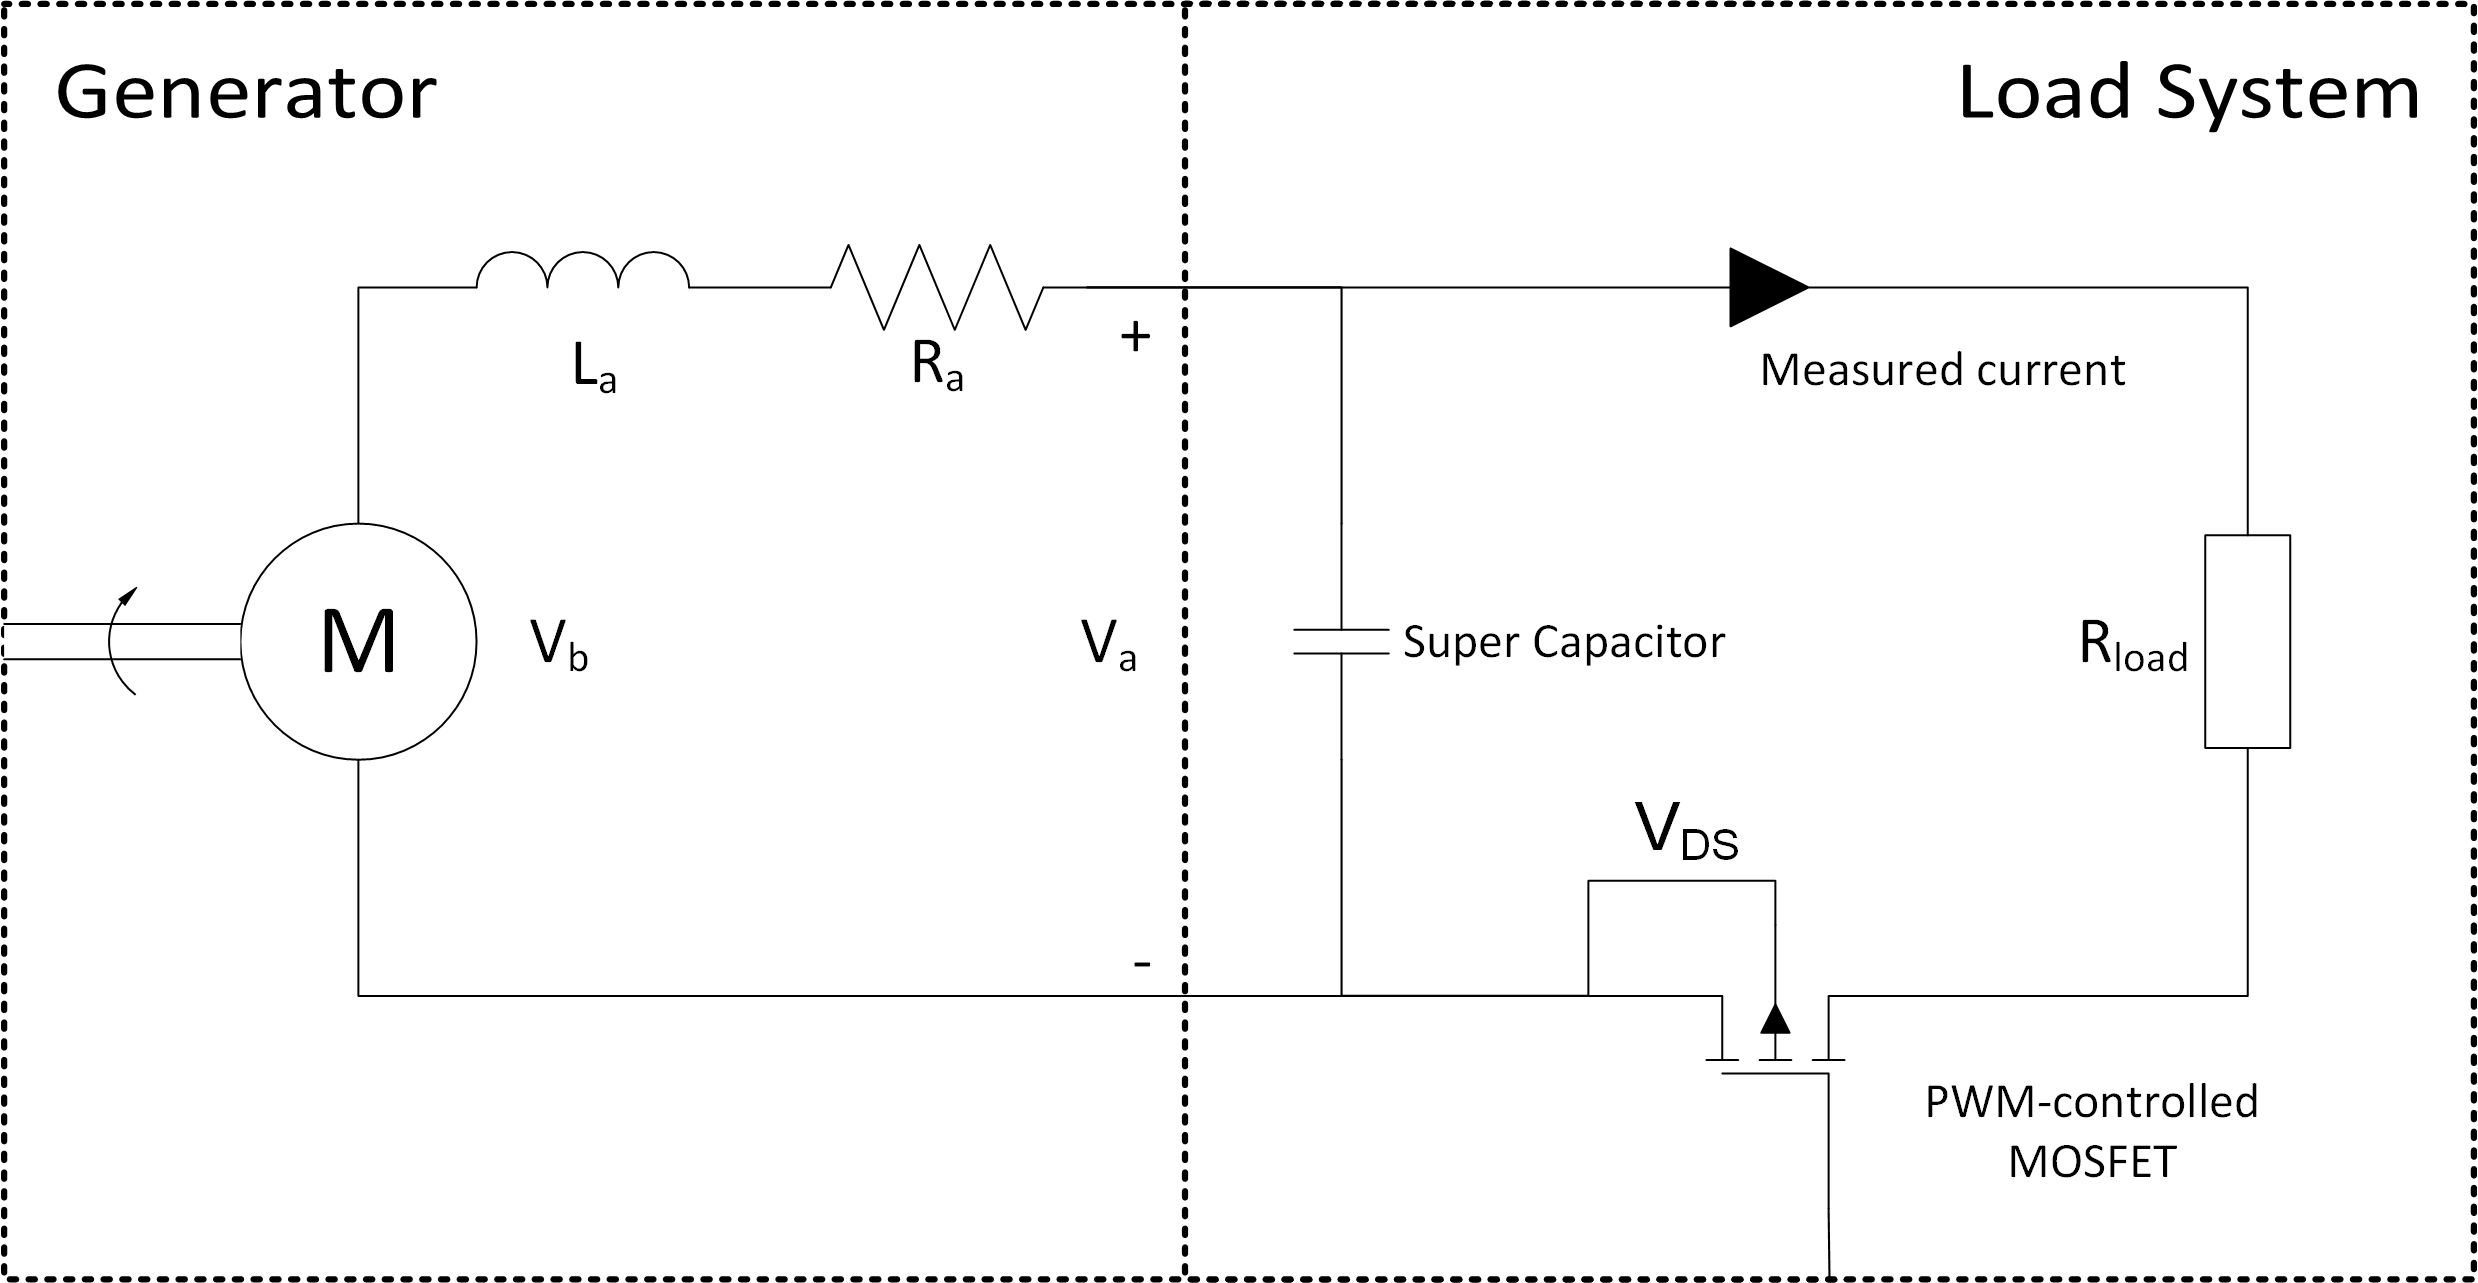
\includegraphics[width=0.7\linewidth]{Hardware/Pictures/LoadSystem}
	\caption{Connection between Generator and Load System}
	\label{fig:Load_System}
\end{figure}

It is assumed that the DC-generator's internal armature can be modelled using a voltage source in series with an inductor and a resistor. The voltage generated by the armature V\textsubscript{b} is proportional to the Generator's rotational velocity. The generated voltage over the armature's resistor will cause a current to flow.

This means that if the Generator's rotational speed is exposed to a  sudden change it will produce a large voltage-drop over the armature's inductor. This voltage will depend on the armature's inductance L\textsubscript{a} and can be calculated as:
\begin{equation}
	V_{La} = L_a \cdot \frac{di}{dt}
\end{equation}
Thus resulting in the fact that a very sudden change in rotational speed could cause a damaging voltage to be produced. This is not desirable and the inductive reactance should therefore be countered by a capacitative reactance. This is done by the Super Capacitor.